\subsection{Formalities}

\begin{frame}{\insertsubsection}
	\begin{mycolumns}
		\mynote{Who Are You?}{
			\begin{itemize}
				\item Bachelor student (5 ECTS)
				\item Master student (6 ECTS)
				\item enrolled in one of these courses of study:
				\begin{itemize}
					\item Informatik
					\item Computervisualistik
					\item Wirtschaftsinformatik
					\item Ingenieurinformatik
					\item Digital Engineering
				\end{itemize}
				\item looking for an elective subject \deutsch{Wahlpflichtfach (WPF)}
			\end{itemize}
		}
	\mynextcolumn
		\mynote{Who Are We?}{
			\centering
			\parbox{0.45\linewidth}{
				\centering
				\href{https://www.dbse.ovgu.de/Mitarbeiter/Gunter+Saake.html}{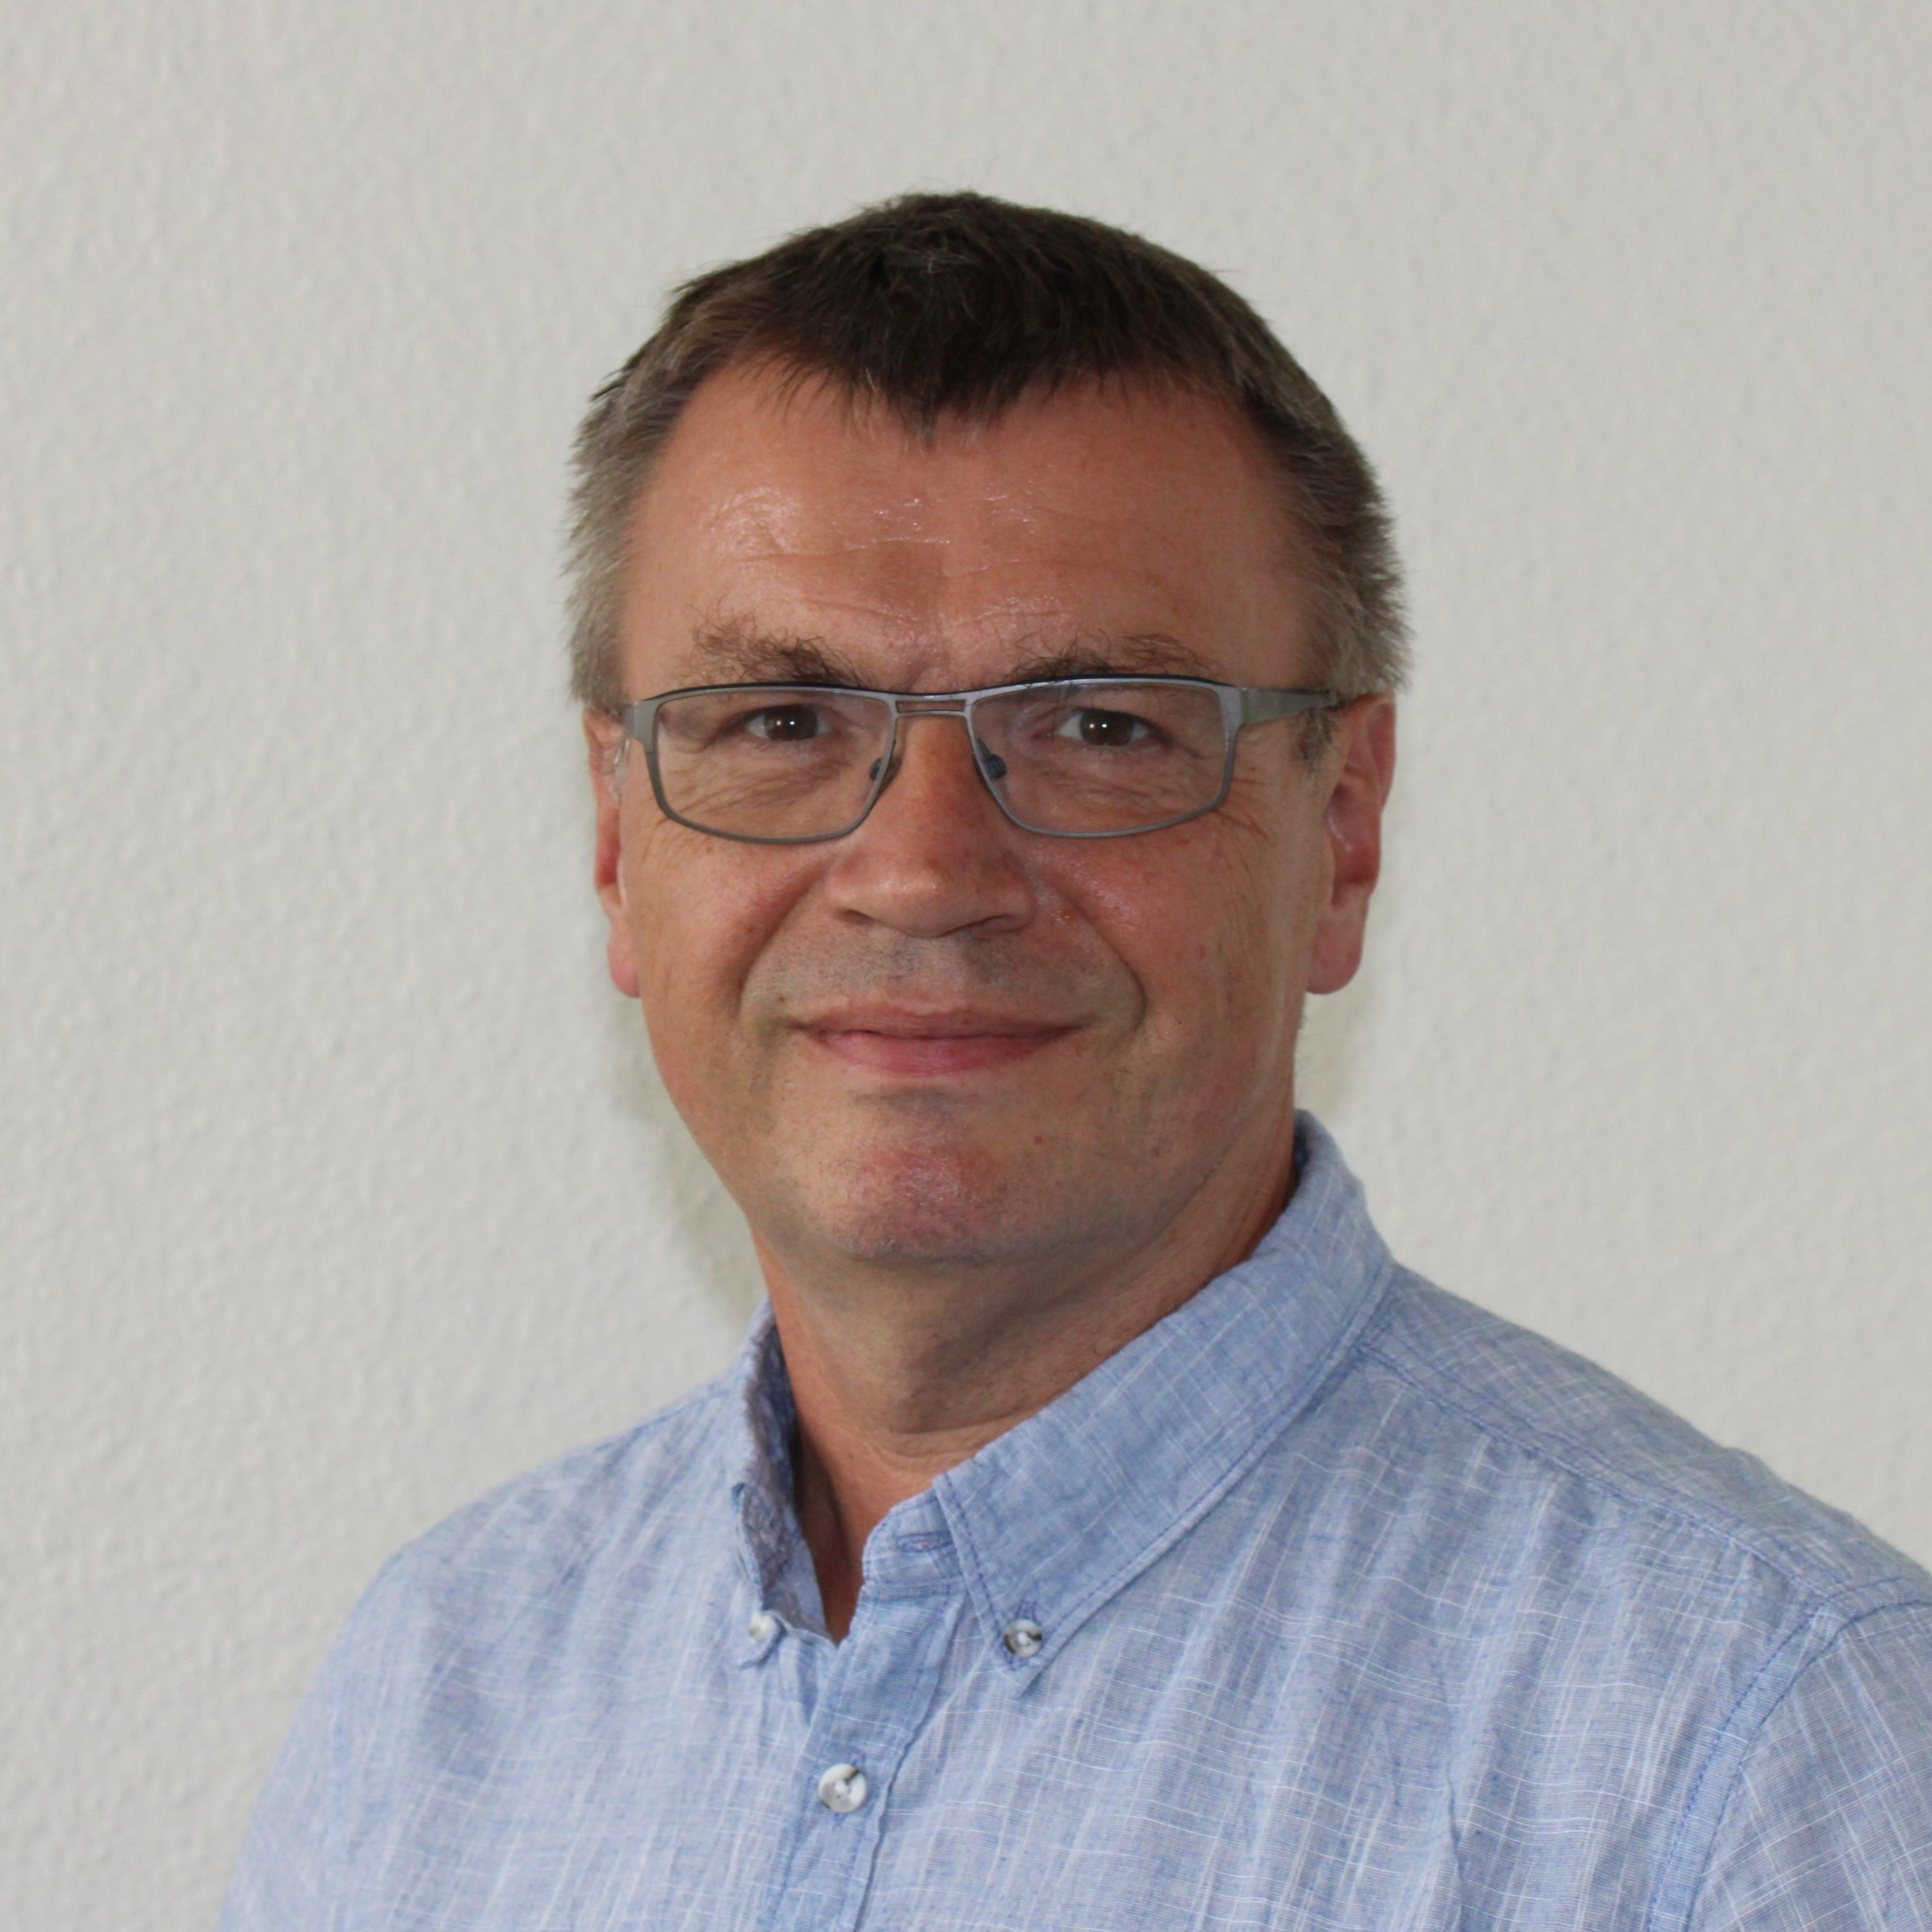
\includegraphics[width=\linewidth]{gunter-saake}}\\[.5ex]
				\href{https://www.dbse.ovgu.de/Mitarbeiter/Gunter+Saake.html}{\emph{Gunter Saake}}\\[.5ex]
				\small professor for databases and software engineering\\[.5ex]
				FeatureIDE project manager
			}
			\parbox{0.45\linewidth}{
				\centering
				\href{https://www.dbse.ovgu.de/Mitarbeiter/Elias+Kuiter.html}{
\includegraphics[width=0.75\linewidth]{elias-kuiter}}\\[.5ex]
				\href{https://www.dbse.ovgu.de/Mitarbeiter/Elias+Kuiter.html}{\emph{Elias Kuiter}}\\[.5ex]
				\small PhD student in feature-model analysis\\[.5ex]
				FeatureIDE core developer
			}
		}
	\end{mycolumns}
\end{frame}

\begin{frame}{\insertsubsection}
	\begin{mycolumns}
		\mynote{Lecture}{
			\begin{itemize}
				\item once per week (2 SWS)
				\begin{itemize}
					\item on \emph{Wednesday}, 09.15am--10.45am
					\item in room G40B-326
					\item starts on October 11
				\end{itemize}
				\item usually held by Gunter
				\item \emph{slides} are handed out in \href{https://elearning.ovgu.de/course/view.php?id=13228}{Moodle}
				\item guest lectures planned:
				\begin{itemize}
					\item industry talk around Christmas
					\item research talk at end of January
				\end{itemize}
			\end{itemize}
		}
	\mynextcolumn
		\mynote{Exercise}{
			\begin{itemize}
				\item once per week (2 SWS)
				\begin{itemize}
					\item on \emph{Tuesday}, 09.15am--10.45am
					\item in room G40B-326
					\item starts on October 18
				\end{itemize}
				\item usually held by Elias
				\item \emph{exercise sheets} are handed out 1 week in advance in \href{https://elearning.ovgu.de/course/view.php?id=13228}{Moodle}
				\item 2 weeks time to work on \emph{practical tasks}
				\item lab exercise planned for end of January
			\end{itemize}
		}
	\end{mycolumns}
\end{frame}

\begin{frame}{\insertsubsection}
	\begin{mycolumns}
		\mynote{Exam Eligibility \deutsch{Prüfungszulassung}}{
			\begin{itemize}
				\item 60\% of all normal tasks \deutsch{Votierungspunkte}
				\item 70\% for Master students
				\item 3 presentation points \deutsch{Vortragspunkte}
				\item all practical tasks (in teams of 2--3 students)
			\end{itemize}
		}
		\mynote{Exam}{
			\begin{itemize}
				\item oral exam ($\approx 20$ minutes)
				\item 1--2 exam days in February or March
				\item to get an ungraded performance \deutsch{Schein}, you have to pass the exam
				\item consultation in the last lecture
			\end{itemize}
		}
	\mynextcolumn
		\mynote{Further Studies}{
			\begin{itemize}
				\item Bachelor/Master thesis
				\item individual project
				\item seminar or software project in summer term % FeatJAR software project or proseminar on advanced language concepts
			\end{itemize}
			\ldots{} consult with us!
		}
	\end{mycolumns}
\end{frame}